\documentclass[12pt]{article}
\usepackage{amssymb}
\usepackage[UTF8]{ctex}
\usepackage{geometry}
\usepackage{units}
\usepackage{pifont}
\geometry{
	a4paper,
	total={150mm,237mm},
	left=30mm,
	top=27mm,
	}
\usepackage{amsmath}
\usepackage{enumerate}
\usepackage{lipsum}
\usepackage{graphicx}
\usepackage{hyperref}
\usepackage{indentfirst}
\usepackage[graphicx]{realboxes}
\usepackage{booktabs}
\usepackage{cases}
\usepackage{subfig}  
\usepackage{float}
\usepackage{pythonhighlight}

\setlength{\parindent}{2em}
\title{HW12}
\author{姓名:陈锐林,学号:21307130148}

\begin{document}
\maketitle
\begin{Large}
    \noindent Chapter41-FFS\\
\end{Large}
Question1:\par
由题意可以知道,in.largefile里只有一行命令"file /a 40";这意味着该文件是放在root下,即第一行开始的。如果我们不使用-L标志,数据块就会从第一行开始堆叠排放,如下左图;而如果使用-L 4,每个gruop都占4个坑,如下右图。
\begin{figure}[!h]
    \centering
    \subfloat[no -L]{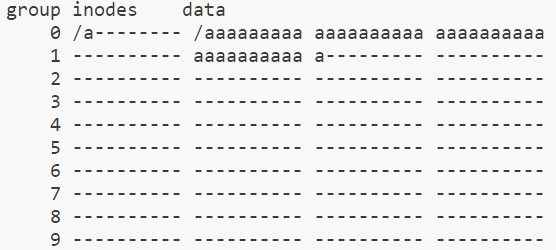
\includegraphics[width=0.46\textwidth]{lab12-1.jpg} \label{X}}
    \hfill
    \subfloat[-L 4]{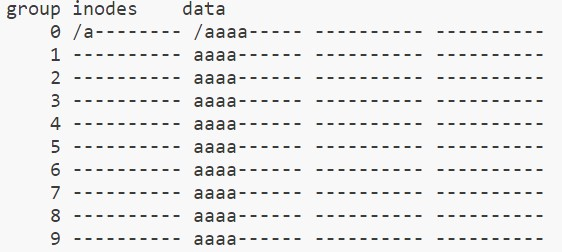
\includegraphics[width=0.46\textwidth]{lab12-2.jpg} \label{Y}}
\end{figure}\\
Question2:-L 30 和 -L 4的意义是一样的;即每行分配30个位置。但是因为文件a只有40的大小,因此排到第二行多11个就停止了,如下图。
\begin{figure}[H]
    \centering
    \includegraphics*[width=0.7\textwidth]{hw12-3.jpg}
\end{figure}
\noindent Question4: 首先分析in.manyfiles内的文件,有三种;一是直接归属于root的,还有分别属于子目录j和t的。那么显然每一类的文件应该在同一组内,而且能发现,这里文件大小都不大;一组的数据块完全放得下。所以最后结果如下图所述,不同目录下的文件放在同一group。
\newpage
\begin{figure}[H]
    \centering
    \includegraphics*[width=0.6\textwidth]{hw12-4.jpg}
\end{figure}
\vspace*{2em}
\begin{Large}
    \noindent Chapter42-Journal\\
\end{Large}
Question1:\par
(1)首先观察通过指令 fsck.py -D生成的如下文件系统。inode中的"[f a:-1]"表示有俩个文件为空。而观察中的首项(根目录),排除与后面有连接的g和w,m和z应该是两个文件名;inode中的"[d a:0]"是根目录,"[d a:12]"和"[d a:6]"是两个目录项,分别对应data中的数据块,再根据前面剩下w和g,可以得到目录名;
最后注意到g下还有"(s,15)",可知g/s也是一个文件。汇总结果,directory: "/","/g","/w";file: "/m","/z","/g/s"。
\begin{figure}[H]
    \centering
    \includegraphics*[width=1\textwidth]{hw12-5.jpg}
\end{figure}
(2)对于其他随机种子,-s 1生成如下;类似的可得结果。directory: "/","/a","/m"(先找到与后面的数据块有连接的a和m,如"(m,7)"和"(.,7)"匹配);file: "/g", "/m/m","/m/e","/a/r","/a/w"。(接着找到目录下的文件)
\begin{figure}[H]
    \centering
    \includegraphics*[width=1\textwidth]{hw12-6.jpg}
\end{figure}
(3)对随机种子,-s 2生成如下;结果也可得。directory: "/","/c","/c/o","/c/o/u"。(现在根目录找到下一级目录c,接着再在c的项中找到o,以此类推);file: "/c/o/q",\\"/c/o/u/q","/c/o/u/e"。
\begin{figure}[H]
    \centering
    \includegraphics*[width=1\textwidth]{hw12-7.jpg}
\end{figure}
\newpage
(4)对随机种子,-s 3生成如下;结果也可得。directory: "/","/r","/r/s";file: "/f","/x"。
\begin{figure}[H]
    \centering
    \includegraphics*[width=1\textwidth]{hw12-8.jpg}
\end{figure}
\noindent Question2:\par (1)运行指令 fsck.py -S 1后,能得到如下结果。能发现问题出在inode bitmap上,按照题目中的[f a:-1 r:2]来看,inode bitmap的第十三位不应该是0,该是1。(2)修改位图,以改变其标识,让它存在。
\begin{figure}[H]
    \centering
    \includegraphics*[width=1\textwidth]{hw12-9.jpg}
\end{figure}
\begin{Large}
    \noindent Chapter43-LFS\\
\end{Large}
Question1:\par
(1)能看到下面出现了ku3和qg9,所以应该进行create file这俩个文件。中间有个区域(如下图)正好对应剩下的一句命令,由imap和size(ptrs)的变化可知,应该是写了ku3,offset为7,size为4。总结如下: create file /ku3 
write file  /ku3 \;\;\; offset=7 size=4 \;\;\;
create file /qg9 
(2)就三条指令,顺序是显然的。(3)最后活跃的块应该包括:临界区,qg9相关,ku3写相关的。即0,8,9,11,12,13,14。(4)当将-n调整为5后,很明显发现工作量变大,这时共23各块,且有新的文件引入,并且操作类型应该也是变得更复杂的;不单单只是create和write。(如下图)
\begin{figure}[H]
    \centering
    \includegraphics*[width=0.6\textwidth]{hw12-10.jpg}
\end{figure}
\begin{figure}[H]
    \centering
    \includegraphics*[width=0.6\textwidth]{hw12-11.jpg}
\end{figure}
\end{document}